\documentclass{beamer}

\usepackage[T1]{fontenc}
\usepackage[utf8]{inputenc}
\usepackage[american]{babel}
\usepackage{amsmath,amssymb,amsthm}
\usepackage{tikz,pgflibraryarrows,pgflibraryplotmarks,pgflibrarysnakes,pgflibraryshapes}
\usepackage{tikzsymbols}
\usepackage[backend=biber,citestyle=authoryear-comp,bibstyle=beamer,doi=false,isbn=false,url=false,maxnames=10]{biblatex}
\usepackage[nosfdefault]{comicneue}
\bibliography{defeo}

\mode<presentation>{%
  \usetheme{Boadilla}
}
\beamertemplatenavigationsymbolsempty
\usecolortheme[RGB={110,117,124}]{structure}
\setbeamercolor*{title}{fg=white!50!black}
\setbeamercolor*{titlegraphic}{fg=white!20!black}

\usepackage{sourcesanspro}
\usepackage[amssymb,amsfonts]{concmath}
\usefonttheme[onlymath]{serif}

\renewcommand{\emph}[1]{{\usebeamercolor[fg]{structure}#1}}

%\let\footcite\footnote

\newcommand{\C}{\mathbb{C}}
\newcommand{\R}{\mathbb{R}}
\newcommand{\Z}{\mathbb{Z}}
\newcommand{\N}{\mathbb{N}}
\newcommand{\Q}{\mathbb{Q}}
\newcommand{\F}{\mathbb{F}}
\renewcommand{\O}{\mathcal{O}}
\newcommand{\tildO}{\mathcal{\tilde{O}}}
\newcommand{\End}{\operatorname{End}}
\newcommand{\chr}{\operatorname{char}}
\newcommand{\Cl}{\operatorname{Cl}}
\renewcommand{\a}{{\mathfrak{a}}}
\renewcommand{\b}{{\mathfrak{b}}}
\newcommand{\cyc}[1]{{\langle #1 \rangle}}
\newcommand{\ord}{\operatorname{ord}}

\usetikzlibrary{matrix,decorations,decorations.text,calc,arrows,snakes,shapes,positioning}

\pgfkeys{/triangle/.code=\tikzset{x={(-0.5cm,-0.866cm)},y={(1cm,0cm)}}}
\pgfkeys{/lattice/.code n args={4}{\tikzset{cm={#1,#2,#3,#4,(0,0)}}}}

\newcommand{\axes}[4]{
  \clip (#1,#3) rectangle (#2,#4);
  \draw [thin, gray, -latex] (#1,0) -- (#2,0);% Draw x axis
  \draw [thin, gray, -latex] (0,#3) -- (0,#4);% Draw y axis
}

\newcommand{\lattice}[2]{
  \draw[style=help lines,dashed] (#1-1,#1-1) grid[step=1] (#2+1,#2+1);
  \foreach \x in {#1,...,#2}{
    \foreach \y in {#1,...,#2}{
      \node[draw,circle,inner sep=2pt,fill] at (\x,\y) {};
      % Places a dot at those points
    }
  }
}

\newcommand{\bl}[1]{\textcolor{blue}{#1}}
\newcommand{\rd}[1]{\textcolor{red}{#1}}
\newcommand{\gr}[1]{\textcolor{green}{#1}}

% This command defines a triangle of dots of given height
\newcommand{\dottriangle}[2][\i-\j]{%
  \foreach \i in {0,...,#2} {%
    \foreach \j in {0,...,\i} {%
      \draw(\i,\j) node{#1};%
    }%
  }}


\title[Isogeny based cryptography]{Isogeny based crypto: what's under the hood?}
\author{Luca De Feo}
\date[ENMSE, Nov 15, 2018]{Nov 15, 2018, École des Mines de Saint-Étienne, Gardanne}
\institute[UVSQ]{Université Paris Saclay -- UVSQ}

\begin{document}

\frame[plain]{
  \begin{tikzpicture}[overlay]
    \node[opacity=0.2] at (10,5) {
      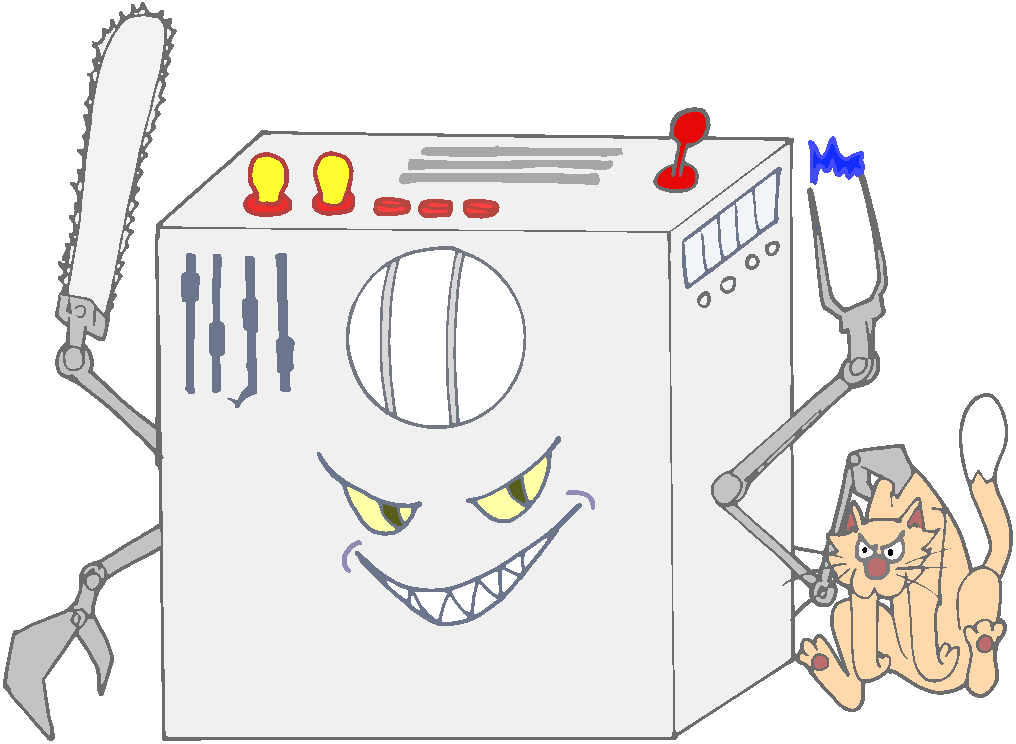
\includegraphics[height=4\textheight]{qc-color}
    };
  \end{tikzpicture}
  \vspace{-2.5cm}
  \usebeamercolor[fg]{titlegraphic}
  {\bf \titlepage}
}

%% 

\begin{frame}{Elliptic curves}

  Let \emph{$E \;:\; y^2 = x^3 + ax + b$} be an elliptic curve\dots

  \begin{center}
    \begin{tikzpicture}[domain=-2.4566:4,samples=100]
      \newcount\rotate
      \animate<2-6>
      \animatevalue<2-6>{\rotate}{0}{90}
      \begin{scope}[rotate=-\the\rotate]
        \draw plot (\x,{0.5*sqrt(\x*\x*\x-4*\x+5)});
        \draw plot (\x,{-0.5*sqrt(\x*\x*\x-4*\x+5)});
      \end{scope}
      
      \begin{uncoverenv}<1>
        \begin{scope}[yscale=1/2]
          \draw[thin,gray,-latex] (0,-7) -- (0,7);
          \draw[thin,gray,-latex] (-3,0) -- (4,0);
          
          \draw (-3,1) -- (4,8/3+3);
          \begin{scope}[every node/.style={draw,circle,inner sep=1pt,fill},cm={1,2/3,0,0,(0,3)}]
            \node at (-2.287980,0) {};
            \node at (-0.535051,0) {};
            \node at (3.267475,0) {};
          \end{scope}
          \begin{scope}[every node/.style={yshift=0.3cm},cm={1,2/3,0,0,(0,3)}]
            \node at (-2.287980,0) {$P$};
            \node at (-0.535051,0) {$Q$};
            \node at (3.267475,0) {$R$};
          \end{scope}
          \draw[dashed] (3.267475,3.267475*2/3+3) -- (3.267475,-3.267475*2/3-3) 
          node[draw,circle,inner sep=1pt,fill] {}
          node[xshift=-0.1cm,anchor=east] {$P+Q$};
        \end{scope}
      \end{uncoverenv}
    \end{tikzpicture}
  \end{center}
\end{frame}

%%

\begin{frame}{Elliptic curves}
  \transdissolve
  \centering
  
\includegraphics[height=0.7\textheight]{ec-happy}

  \Large\bf I power 70\% of WWW traffic!
\end{frame}

%% 

\begin{frame}{The QUANTHOM Menace}
  \centering
  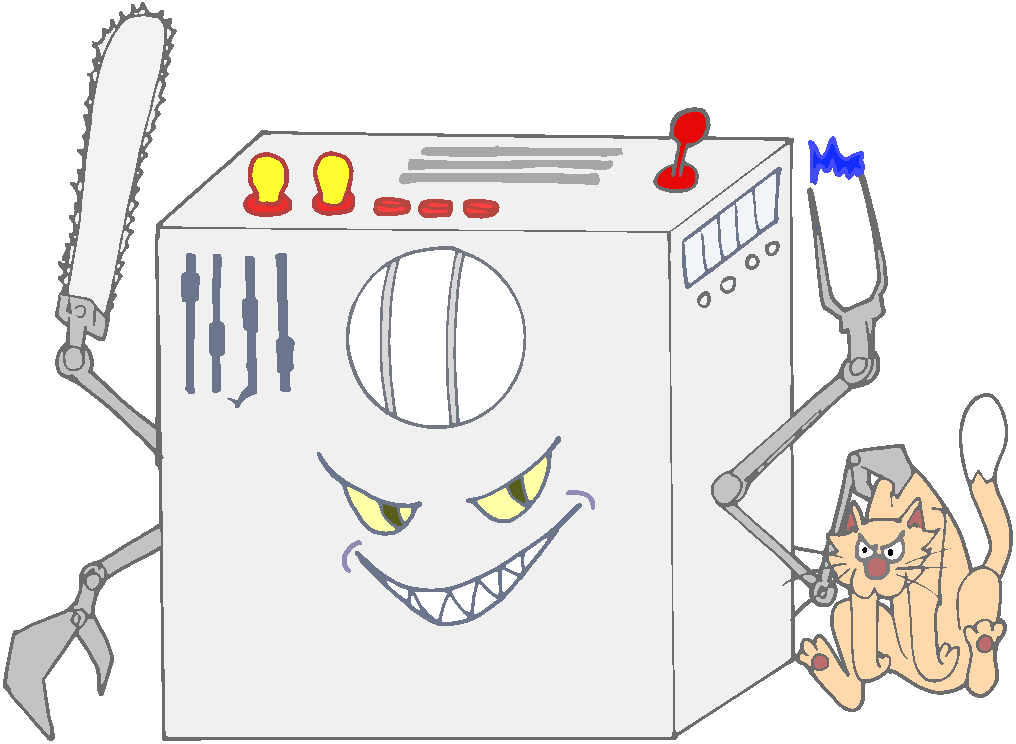
\includegraphics[height=0.7\textheight]{qc-color}
\end{frame}

%% 

\begin{frame}{Post-quantum cryptographer?}
  \centering
  \includegraphics[height=0.7\textheight]{ec-broke}
\end{frame}

%%

\begin{frame}{Elliptic curves of the world, UNITE!}
  \centering
  \begin{tikzpicture}
    \foreach \x/\y in {0/-0.5,4/2,8/-1}{
      \node at (\x,\y) {\includegraphics[height=3cm]{ec-banderole}};
    }
    \foreach \x/\y in {1/3,4.5/-1,7/3}{
      \node at (\x,\y) {
\includegraphics[height=3.5cm]{ec-sign}};
    }
    \color{teal!70!blue}\itshape\bfseries\comicneue
    \node[rotate=-3] at (5.9,3.6) {\parbox{0pt}{QUOUSQUE\\QUANTUM?}};
    \node[rotate=-3] at (3.6,-0.4) {\parbox{0pt}{QUANTUM\\SUFFICIT!}};
  \end{tikzpicture}
\end{frame}

%%

\begin{frame}{And so, they found a way around the Quanthom...}
  \centering
  \begin{tikzpicture}
    \comicneue\itshape
    \node at (0,0) {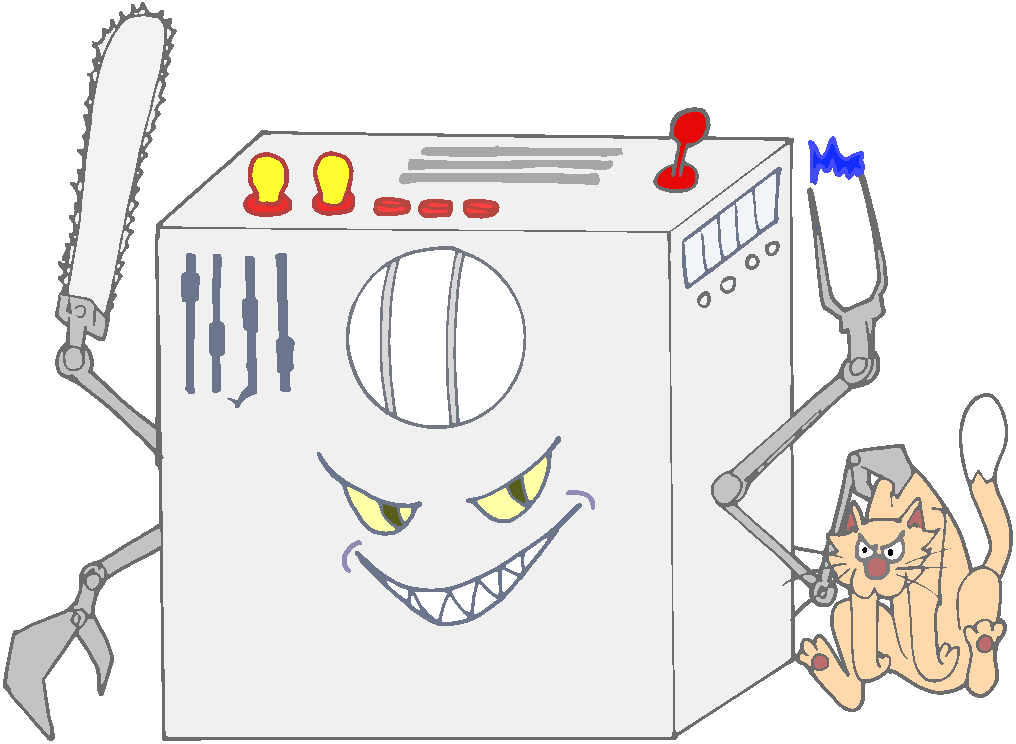
\includegraphics[height=2.5cm]{qc-color}};
    
    \node(E0) at (-5,0) {
\includegraphics[height=1cm]{ec-happy}};

    \uncover<2->{
      \node(EA) at (0,3.5) {
\includegraphics[height=1cm]{ec-happy}};
      \node(EB) at (0,-3.5) {
\includegraphics[height=1cm]{ec-happy}};
      \draw[->,decorate,decoration=snake] (E0) to (EA);
      \draw[->,decorate,decoration=snake] (E0) to (EB);
      \node[right=0.3cm of EA] {\bl{Public curve}};
      \node[right=0.3cm of EB] {\bl{Public curve}};
    }
    \uncover<3>{
      \node(ES) at (5,0) {
\includegraphics[height=1cm]{ec-happy}};
      \draw[->,decorate,decoration=snake] (EA) to (ES);
      \draw[->,decorate,decoration=snake] (EB) to (ES);
      \node[below=1em of ES] {\rd{Shared secret}};
    }
  \end{tikzpicture}
\end{frame}

%%

\begin{frame}{A brief history of isogeny-based key exchange}
  \begin{description}
  \item[1996] Couveignes introduces \emph{Hard Homogeneous
      Spaces}. His work stays unpublished for 10 years.
  \item[2006] Rostovtsev \& Stolbunov independently rediscover
    Couveignes ideas, suggest isogeny-based Diffie--Hellman as a
    \emph{quantum-resistant} primitive.
  \item[2006-2010] Other isogeny-based protocols by Teske and Charles,
    Goren \& Lauter.
  \item[2011-2012] D., Jao \& Plût introduce \emph{SIDH}, an
    efficient post-quantum key exchange inspired by Couveignes,
    Rostovtsev, Stolbunov, Charles, Goren, Lauter.
  \item[2017] SIDH is submitted to the NIST competition (with the name
    \emph{SIKE}, only isogeny-based candidate).
  \item[2018] D., Kieffer \& Smith \textit{resurrect} the
    Couveignes--Rostovtsev--Stolbunov protocol, Castryck, Lange,
    Martindale, Panny \& Renes publish an efficient variant named
    \emph{CSIDH}.
  \end{description}
\end{frame}

%%

\begin{frame}
  \frametitle{What's an isogeny?}

  Isogenies are just \alert{the right notion\texttrademark{} of
    morphism} for elliptic curves

  \begin{itemize}
  \item Surjective group morphisms.
  \item Algebraic maps (i.e., defined by polynomials).
  \end{itemize}

  (Separable) isogenies $\Leftrightarrow$ finite subgroups:
  \alert{\[0 \to H \to E \overset{\phi}{\to} E' \to 0\]}
  
  \begin{block}{Separable isogenies (write this down, now!)}
    \begin{itemize}
    \item The kernel \emph{$H$} determines the image curve \emph{$E'$}
      up to isomorphism:
      \[\alert{E/H\overset{\text{\tiny def}}{=}E'}.\]
    \item The \emph{degree} of \emph{$\phi:E\to E/H$} is the
      \emph{size} of the kernel \emph{$H$}:
      \[\alert{\deg\phi\overset{\text{\tiny def}}{=}\#\ker\phi}.\]
    \end{itemize}
  \end{block}
\end{frame}

%% 

\begin{frame}{Isogenies: an example over $\F_{11}$}
  \begin{tikzpicture}[scale=0.4]
    \begin{scope}
      \node[anchor=center] at (0,7) {$E \;:\; y^2 = x^3 + x$};

      \uncover<-1>{
        \draw[thin,gray] (0,-6) -- (0,6);
        \draw[thin,gray] (-6,0) -- (6,0);
      }

      \foreach \x/\y in {0/0,5/3,-4/3,-3/5,-2/1,-1/3} {
        \draw[blue,fill] (\x,\y) circle (0.2) node(E_\x_\y){}
        (\x,-\y) circle (0.2) node(E_\x_-\y){};
      }

      \uncover<2->{\draw[red,fill] (0,0) circle (0.3);}
    \end{scope}

    \draw[black!10!white,thick] (8,-7) -- +(0,14);
    
    \begin{scope}[shift={(16,0)}]
      \node at (0,7) {$E' \;:\; y^2 = x^3 - 4x$};

      \uncover<-1>{
        \draw[thin,gray] (0,-6) -- (0,6);
        \draw[thin,gray] (-6,0) -- (6,0);
      }

      \foreach \x/\y in {0/0,2/0,3/2,4/2,6/4,-2/0,-1/5} {
        \draw[color=blue,fill] (\x,\y) circle (0.2) node(F_\x_\y){}
        (\x,-\y) circle (0.2) node(F_\x_-\y){};
      }
    \end{scope}

    \begin{scope}[color=red,-latex,dashed]
      \begin{uncoverenv}<2->
        \path
        (E_5_3) edge (F_3_2)
        (E_-4_3) edge (F_4_-2)
        (E_-3_5) edge (F_4_2)
        (E_-2_1) edge (F_3_-2)
        (E_-1_3) edge (F_-2_0);
      \end{uncoverenv}
      \begin{uncoverenv}<2->
        \path
        (E_5_-3) edge (F_3_-2)
        (E_-4_-3) edge (F_4_2)
        (E_-3_-5) edge (F_4_-2)
        (E_-2_-1) edge (F_3_2)
        (E_-1_-3) edge (F_-2_0);
      \end{uncoverenv}
    \end{scope}
  \end{tikzpicture}
  
  \begin{columns}
    \begin{column}{0.5\textwidth}
      \[\phi(x,y) = \left(\frac{x^2 + 1}{x},\quad y\frac{x^2-1}{x^2}\right)\]
    \end{column}
    \begin{column}{0.5\textwidth}
      \begin{itemize}
      \item<2-> Kernel generator in \alert{red}.
      \item<2-> This is a degree $2$ map.
      \item<2-> Analogous to $x\mapsto x^2$ in $\F_q^*$.
      \end{itemize}
    \end{column}
  \end{columns}
\end{frame}

%%

\begin{frame}
  \frametitle{Isogeny graphs}
  
  \vspace{-2mm}

  \begin{columns}
    \begin{column}{0.65\textwidth}
      We look at the graph of elliptic curves with isogenies \emph{up
        to isomorphism}.  We say two \alert{isogenies} $\phi,\phi'$
      are \alert{isomorphic} if:
    \end{column}
    \begin{column}{0.3\textwidth}
      \begin{center}
        \begin{tikzpicture}[node distance=4em]
          \node(E){$E$}; 
          \node(E1)[right of=E]{$E'$};
          \node(E2)[below of=E1]{$E'$};
          \scriptsize
          \path[->] (E) edge node[auto]{$\phi$} (E1);
          \path[->] (E) edge node[auto,swap]{$\phi'$} (E2);
          \path[<->] (E1) edge node[rotate=270] {\large$\widetilde{}$} (E2);
        \end{tikzpicture}
      \end{center}
    \end{column}
  \end{columns}

  \emph{Example:} Finite field, ordinary case, graph of isogenies of degree $3$.

  \begin{center}
    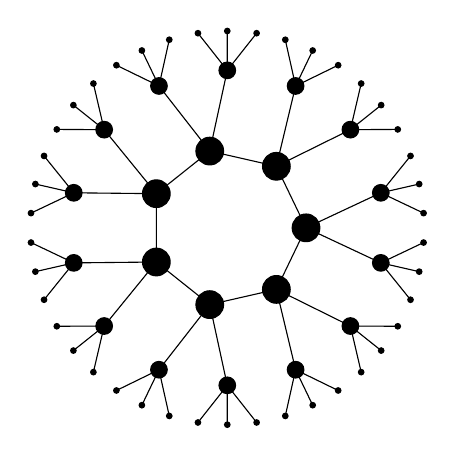
\begin{tikzpicture}[]
      \begin{scope}
        \def\crater{7}
        \foreach \i in {1,...,\crater} {
          \draw[fill] (360/\crater*\i:1cm) circle (5pt);
          \draw (360/\crater*\i : 1cm) -- (360/\crater*\i+360/\crater : 1cm);
          \foreach \j in {-1,1} {
            \draw[fill] (360/\crater*\i : 1cm) -- (360/\crater*\i + \j*360/\crater/4 : 2cm) circle (3pt);
            \foreach \k in {-1,0,1} {
              \draw[fill] (360/\crater*\i + \j*360/\crater/4 : 2cm) --
              (360/\crater*\i + + \j*360/\crater/4 + \k*360/\crater/6 : 2.5cm) circle (1pt);
            }
          }
        }
      \end{scope}
    \end{tikzpicture}
  \end{center}
\end{frame}

%%

\begin{frame}
  \frametitle{Structure of the graph}
  
  \begin{theorem}[Serre-Tate]
    Two curves are isogenous over a finite field $k$ if and only if
    they have the \alert{same number of points} on $k$.
  \end{theorem}
  \vspace{-0.6em}
  \begin{block}{The graph of isogenies of \alert{prime} degree \alert{$\ell\ne p$}}
    \small
    \vspace{-1em}
    \begin{tabular}{p{0.17\textwidth} p{0.8\textwidth}}
      \raggedright
      \emph{Ordinary case (isogeny volcanoes)}
      & \vspace{-1em}
        \begin{itemize}
          \setlength\itemsep{-0.6ex}
        \item Nodes can have degree \emph{$0,1,2$} or \emph{$\ell+1$}.
          \begin{itemize}
          \item  For $\sim 50\%$ of the primes $\ell$, graphs are just isolated
            points;
          \item For other $\sim 50\%$, graphs are $2$-regular;
          \item other cases only happen for finitely many $\ell$'s.
          \end{itemize}
        \end{itemize}
      \\[-1.4em]
      \raggedright
      \emph{Supersingular case ($\F_p$)}
      & \vspace{-1.2em}
        \begin{itemize}
          \setlength\itemsep{-0.6ex}
        \item If $\ell=2$ nodes have degree $1$, $2$ or $3$;
        \item For $\sim 50\%$ of $\ell$, graphs are isolated points;
        \item For other $\sim 50\%$, graphs are $2$-regular;
        \end{itemize}
      \\[-1em]
      \raggedright
      \emph{Supersingular case ($\F_{p^2}$)}
      & \vspace{-1em}
        \begin{itemize}
          \setlength\itemsep{-0.6ex}
        \item The graph is \emph{$\ell+1$-regular}.
        \item There is a \alert{unique (finite) connected component} made
          of all supersingular curves with the same number of points.
        \end{itemize}
    \end{tabular}
    \vspace{-1.5em}
  \end{block}
\end{frame}

%%

\begin{frame}
  \frametitle{Complex multiplication graphs}
  \begin{center}
    \begin{tikzpicture}
      \begin{scope}
        \def\crater{12}
        \def\jumpa{-8}
        \def\jumpb{9}
        \def\diam{3cm}

        \foreach \i in {1,...,\crater} {
          \uncover<2->{\draw[blue] (360/\crater*\i : \diam) to[bend right] (360/\crater*\i+360/\crater : \diam);}
          \uncover<3->{\draw[red] (360/\crater*\i : \diam) to[bend right] (360/\crater*\i+\jumpa*360/\crater : \diam);}
          \uncover<4->{\draw[green] (360/\crater*\i : \diam) to[bend right=50] (360/\crater*\i+\jumpb*360/\crater : \diam);}
        }
        \foreach \i in {1,...,\crater} {
          \draw[fill] (360/\crater*\i: \diam) circle (2pt) +(360/\crater*\i: 0.4) node{$E_{\i}$};
        }
      \end{scope}
      \begin{scope}[xshift=4cm]
        \draw (0,2.5) node[anchor=west] {\parbox{4cm}{%
            Vertices are elliptic curves \emph{with complex
              multiplication by $\O_K$} (i.e., $\End(E)\simeq\O_K\subset\Q(\sqrt{-D})$).\\
            \uncover<2->{Edges are \emph{horizontal isogenies} of
              bounded prime degree.}  }};
      
        \uncover<2->{\draw[blue] (0,0) -- (0.5,0)
          (0.5,0) node[anchor=west] {degree $2$};}
        \uncover<3->{\draw[red] (0,-1) -- (0.5,-1) (0.5,-1)
          node[anchor=west] {degree $3$};}
        \uncover<4->{\draw[green]
          (0,-2) -- (0.5,-2) (0.5,-2) node[anchor=west] {degree $5$};}

        \uncover<5->{\draw (0,-3) node[anchor=west] {\parbox{4cm}{%
              Isomorphic to a \emph{Cayley graph of $\Cl(\O_K)$}.}};}
      \end{scope}
    \end{tikzpicture}
  \end{center}
\end{frame}

%% 

{
  \newcommand{\myedge}[3]{
    \draw[#3] (360/\crater*#1 : \diam) to[bend right] (360/\crater*#2 : \diam);
  }

\begin{frame}
  \frametitle{Rostovtsev \& Stolbunov key exchange (CRS)}

  \begin{columns}
    \begin{column}{0.55\textwidth}
      \begin{tikzpicture}
        \begin{scope}
          \def\crater{12}
          \def\jumpa{-8}
          \def\jumpb{9}
          \def\diam{2.5cm}
          
          \foreach \i in {1,...,\crater} {
            \pgfmathparse{int(mod(2^\i,13))}
            \let\exp\pgfmathresult
            \draw[fill] (360/\crater*\i: \diam) circle (2pt);
          }
          \uncover<2,6->{
            % Alice 1
            \myedge{0}{1}{blue}\myedge{1}{5}{red}\myedge{5}{6}{blue}\myedge{6}{3}{green}
          }
          \uncover<3,5>{
            % Bob 1
            \begin{scope}[dashed,thick]
              \myedge{0}{4}{red}\myedge{4}{8}{red}\myedge{8}{5}{green}\myedge{5}{6}{blue}
            \end{scope}
          }
          \uncover<5>{
            % Alice 2
            \myedge{6}{7}{blue}\myedge{7}{11}{red}\myedge{11}{0}{blue}\myedge{0}{9}{green}
          }
          \uncover<6->{
            % Bob 2
            \begin{scope}[dashed,thick]
              \myedge{3}{7}{red}\myedge{7}{11}{red}\myedge{11}{8}{green}\myedge{8}{9}{blue}
            \end{scope}
          }

          \draw (0 : \diam + 0.4cm) node {$E$};
          \uncover<2->{\draw (360/\crater*3 : \diam + 0.4cm) node {$\a*E$};}
          \uncover<3->{\draw (360/\crater*6 : \diam + 0.6cm) node {$\b*E$};}
          \uncover<5->{\draw (360/\crater*9 : \diam + 0.4cm) node {$\a\b*E\uncover<6->{=\b\a*E}$};}
        \end{scope}
      \end{tikzpicture}  
    \end{column}    
    \begin{column}{0.45\textwidth}
      \textbf{Public parameters:}
      \begin{itemize}
      \item A starting curve \emph{$E/\F_p$} with \emph{CM by $\O_K$};
      \item A set of ideals of small norm \emph{$S\subset\Cl(\O_K)$}.
      \end{itemize}
      \begin{enumerate}
      \item<2-> \textbf{Alice} takes a \alert{secret} random walk
        \emph{$\a=\prod_{\frak s\in S}\frak s^{e_{\frak s}}$}
        defining an isogeny \emph{$E\to \a*E$};
      \item<3-> \textbf{Bob} does the same;
      \item<4-> They publish \emph{$\a*E$} and \emph{$\b*E$};
      \item<5-> \textbf{Alice} repeats her secret walk \emph{$\a$}
        starting from \emph{$\b*E$}.
      \item<6-> \textbf{Bob} repeats his secret walk \emph{$\b$}
        starting from \emph{$\a*E$}.
      \end{enumerate}
    \end{column}
  \end{columns}
\end{frame}
}

%%

\begin{frame}{How to evaluate an isogeny action}
  \begin{description}
  \item[Input:] A degree $\ell$,%
    \hspace{1em} a \textit{direction} (left/right/\dots),%
    \hspace{1em} [a point \emph{$P\in E$}];
  \item[Output:] The curve \emph{$E/H$},%
    \hspace{1em} [the image \emph{$\phi(P)\in E/H$}].
  \end{description}

  \begin{block}{Elkies' algorithm}
    \begin{itemize}
    \item Applies to any curve/degree/kernel;
    \item Complexity \emph{$O(\ell^2)$}, very costly in practice;
    \item Outputs:
      \begin{itemize}
      \item A \emph{kernel polynomial} such that $h(P)=0$ iff $P\in H$;
      \item The \emph{image curve} $E/H$ (using Vélu's formulas).
      \end{itemize}
    \end{itemize}
  \end{block}

  \begin{block}{Direct application of Vélu's formulas}
    \begin{itemize}
    \item Only possible if \emph{$H\subset E(\F_p)$};
      \hspace{4em}($\Leftrightarrow \emph{\ell\mid\#E(\F_p)}$)
    \item Complexity \emph{$O(\ell)$}, very efficient;
    \item Outputs:
      \begin{itemize}
      \item The \emph{image curve} $E/H$.
      \end{itemize}
    \end{itemize}
  \end{block}
\end{frame}

%%

\begin{frame}{CSIDH {\small (pron.: \textit{sea-side})}}
  \begin{block}{Speeding up the CRS key
      exchange \parencite{defeo-kieffer-smith}}
    \begin{itemize}
    \item Choose \emph{$p$} such that \emph{$\ell\mid(p+1)$} for many
      small primes \emph{$\ell$};
    \item Look for random \emph{ordinary} curves such that: \hfill\alert{HARD!}
      \begin{itemize}
      \item \emph{$\ell\mid E(\F_p)$},
      \item technical condition;
      \end{itemize}
    \item Use Vélu's formulas for \emph{those primes $\ell$}.
    \item $\sim$5 minutes for a 128-bit secure key exchange \hfill\alert{\Sadey}
    \end{itemize}
  \end{block}

  \begin{block}{CSIDH \parencite{csidh}}
    \begin{itemize}
    \item Choose \emph{$p$} such that \emph{$\ell\mid(p+1)$} for many
      small primes \emph{$\ell$};
    \item Select a \emph{supersingular} curve \emph{$E/\F_p$},
      automatically \hfill\alert{EASY!}
      \begin{itemize}
      \item \emph{$\#E(\F_p)=p+1$},
      \item technical condition always satisfied;
      \end{itemize}
    \item $\sim$100ms for a 128 bits secure key exchange \hfill\alert{\Smiley}
    \end{itemize}
  \end{block}
\end{frame}

%%

\begin{frame}
  \frametitle{Key exchange with full supersingular graphs (over $\F_{p^2}$)}
  
  \begin{description}
  \item[Good news:] there is no action of a commutative class group.
  \item[Bad news:] there is no action of a commutative class group.
  \item[Idea:] Let \bl{Alice} and \rd{Bob} walk in two
    \emph{different isogeny graphs} on the \emph{same vertex set}.
  \end{description}

  \begin{columns}
    \begin{column}{0.7\textwidth}
      \centering
      \begin{tikzpicture}[scale=1.4]
        \begin{scope}[every node/.style={fill,black,circle,inner sep=2pt}]
          \node at (0,0)  (1){};
          \node at (0,4) (20){};
          \node at (2,1)  (16z){};
          \node at (-2,1)  (81z){};
          \node at (-1,2) (77z){};
          \node at (1,2)  (20z){};
          \node at (-2,3)  (85z){};
          \node at (2,3)  (12z){};
        \end{scope}

        \begin{uncoverenv}<1,3>
          \begin{scope}[blue,every loop/.style={looseness=50}]
            \path (1) edge (20) edge (16z) edge (81z);
            \path (20) edge[loop left] (20) edge[loop right] (20);
            \path (16z) edge (81z) edge (77z);
            \path (81z) edge (20z);
            \path (77z) edge (20z) edge (85z);
            \path (20z) edge (12z);
            \path (12z) edge[bend right=10] (85z) edge[bend left=10] (85z);
          \end{scope}
        \end{uncoverenv}
        
        \begin{uncoverenv}<2->
          \begin{scope}[red]
            \path (1) edge (85z) edge (81z) edge (12z) edge (16z);
            \path (20) edge (85z) edge (77z) edge (20z) edge (12z);
            \path (81z) edge (85z) edge (77z) edge (16z);
            \path (85z) edge (12z);
            \path (12z) edge (16z);
            \path (16z) edge (20z);
            \path (20z) edge[bend right=10] (77z) edge[bend left=10] (77z);
          \end{scope}
        \end{uncoverenv}
      \end{tikzpicture}
    \end{column}
    \begin{column}{0.3\textwidth}
      \small
      \emph{Figure:} \bl{$2$}- and \rd{$3$}-isogeny graphs on $\F_{97^2}$.
    \end{column}
  \end{columns}
\end{frame}

%%

\begin{frame}
  \frametitle{Key exchange with full supersingular graphs (over $\F_{p^2}$)}

  \begin{itemize}
  \item Fix small primes \bl{$\ell_A$}, \rd{$\ell_B$};
  \item \emph{No canonical labeling} of the \bl{$\ell_A$}- and
    \rd{$\ell_B$}-isogeny graphs; \emph{however\dots}
  \end{itemize}

  \begin{center}
    \bf
    Walk of length \bl{$e_A$}\\
    $=$\\
    Isogeny of degree \bl{$\ell_A^{e_A}$}\\
    $=$\\
    Kernel \bl{$\langle P\rangle\subset E[\ell_A^{e_A}]$}
  \end{center}
  
  \begin{center}
    \begin{tikzpicture}
      \begin{scope}
        \draw (0,1.2) node[anchor=east,blue] {$\ker\phi=\cyc{P}\subset E[\ell_A^{e_A}]$};
        \draw (0,0.4) node[anchor=east,red] {$\ker\psi=\cyc{Q}\subset E[\ell_B^{e_B}]$};
        \draw (0,-0.4) node[anchor=east,blue] {$\ker\phi' = \cyc{\rd{\psi}(P)}$};
        \draw (0,-1.2) node[anchor=east,red] {$\ker\psi' = \cyc{\bl{\phi}(Q)}$};
      \end{scope}
      \begin{scope}[xshift=4.5cm,coils/.style={-angle 90,decorate,decoration={coil,aspect=0,amplitude=1pt}}]
        \large
        \node[matrix of nodes, ampersand replacement=\&, column sep=3cm, row sep=1.5cm] (diagram) {
          |(E)| $E$ \& |(Es)| $E/\cyc{\bl{P}}$ \\
          |(Ep)| {$E/\cyc{\rd{Q}}$} \& |(Eps)| {$E/\cyc{\bl{P},\rd{Q}}$}\\
        };
        \path[->,blue] (E) edge[coils] node[auto] {$\phi$} (Es);
        \path[->,blue] (Ep) edge[coils] node[auto,swap] {$\phi'$} (Eps);
        \path[->,red] (E) edge[coils] node[auto,swap] {$\psi$} (Ep);
        \path[->,red] (Es) edge[coils] node[auto] {$\psi'$} (Eps);
      \end{scope}
    \end{tikzpicture}
  \end{center}
\end{frame}

%%

\begin{frame}
  \frametitle{Supersingular Isogeny
    Diffie-Hellman\footcite{jao+defeo2011,defeo+jao+plut12}}

  \vspace{-1cm}

  \begin{columns}
    \begin{column}{0.4\textwidth}
      \begin{block}{}
        \emph{Parameters:}
        \begin{itemize}
          \setlength{\itemsep}{1.5ex}
        \item Prime $p$ such that $p+1 = \bl{\ell_A^a}\rd{\ell_B^b}$;
        \item Supersingular curve \emph{$E\simeq (\Z/(p+1)\Z)^2$};
        \item \bl{$E[\ell_A^a] = \cyc{P_A,Q_A}$};
        \item \rd{$E[\ell_B^b] = \cyc{P_B,Q_B}$}.
        \end{itemize}

        \emph{Secret data:}
        \begin{itemize}
          \setlength{\itemsep}{1.5ex}
        \item \bl{$R_A = m_AP_A + n_AQ_A$},
        \item \rd{$R_B = m_BP_B + n_BQ_B$},
        \end{itemize}
      \end{block}
    \end{column}
    \begin{column}{0.58\textwidth}
      \begin{center}
        \begin{tikzpicture}[coils/.style={-angle 90,decorate,decoration={coil,aspect=0,amplitude=1pt}}]
          \large
          \node[matrix of nodes, ampersand replacement=\&, column sep=4mm, row sep=2cm] (diagram) {
            \& |(1)| $E$ \\
            |(a)| \parbox{1.5cm}{$E/\cyc{\bl{R_A}}$\\\uncover<2->{{\footnotesize $\bl{\phi(}\rd{P_B}\bl{)}\\\bl{\phi(}\rd{Q_B}\bl{)}$}}} \& \&
            |(b)| \parbox{1.5cm}{$E/\cyc{\rd{R_B}}$\\\uncover<2->{{\footnotesize $\rd{\psi(}\bl{P_A}\rd{)}\\\rd{\psi(}\bl{Q_A}\rd{)}$}}}\\
            \normalsize $\frac{E/\cyc{\bl{R_A}}}{\alert{\bl{\phi(}\rd{R_B}\bl{)}}} \simeq$ \&
            |(ab)|  $E/\cyc{\bl{R_A},\rd{R_B}}$ \&
            \normalsize $\simeq \frac{E/\cyc{\rd{R_B}}}{\alert{\rd{\psi(}\bl{R_A}\rd{)}}}$\\
          };
          \small
          \path[blue] (1) edge[coils] node[auto,swap](phia) {$\phi$} (a);
          \path[red] (1) edge[coils] node[auto](phib) {$\psi$} (b);
          \path[red] (a) edge[coils] node[auto,swap](psia){$\psi'$} (ab);
          \path[blue] (b) edge[coils] node[auto](psib){$\phi'$} (ab);
          \uncover<3>{\path[dashed,->] (phia) edge node[auto]{\footnotesize $\bl{\phi(}\rd{R_B}\bl{)}$} (psia);}
          \uncover<3>{\path[dashed,->] (phib) edge node[auto,swap]{\footnotesize $\rd{\psi(}\bl{R_A}\rd{)}$} (psib);}
        \end{tikzpicture}
      \end{center}  
    \end{column}
  \end{columns}
\end{frame}

%%

\begin{frame}{SIKE: Supersingular Isogeny Key Encapsulation}
  \begin{itemize}
  \item Submission to the \emph{NIST PQ competition}:
    \begin{description}
    \item[SIKE.PKE:] El Gamal-type system with \emph{IND-CPA} security
      proof,
    \item[SIKE.KEM:] generically transformed system with
      \emph{IND-CCA} security proof.
    \end{description}
  \item Security levels 1, 3 and 5.
  \item \emph{Smallest communication complexity} among all proposals
    in each level.
  \item \emph{Slowest} among all benchmarked proposals in each level.
  \item A team of 14 submitters, from 8 universities and companies.
  \item Download the package
    \href{https://csrc.nist.gov/CSRC/media/Projects/Post-Quantum-Cryptography/documents/round-1/submissions/SIKE.zip}{\emph{here}}.
  \end{itemize}

  \centering
  \begin{tabular}{l | c c c c c }
    & $p$ & cl. security & q. security & speed & comm.\\
    \hline
    SIKEp503 & $2^{250}3^{159}-1$ & 126 bits & 84 bits & 10ms & 0.4KB\\
    SIKEp751 & $2^{372}3^{239}-1$ & 188 bits & 125 bits & 30ms & 0.6KB\\
    SIKEp964 & $2^{486}3^{301}-1$ & 241 bits & 161 bits & & 0.8KB
  \end{tabular}
\end{frame}

%%

\begin{frame}{CSIDH vs SIDH}
  \centering
  \vspace{-3mm}
  \begin{tabular}{l | c | c}
    & \textbf{CSIDH} & \textbf{SIDH}\\
    \hline
    Speed (NIST 1) & <100ms & $\sim$ 10ms\\
    Public key size (NIST 1) & 64B & 378B\\
    Key compression\footcite{10.1007/978-3-319-79063-3_12} & \\
    \enskip{}\rotatebox[origin=c]{180}{$\Lsh$} speed & & $\sim$ 15ms\footnote{https://twitter.com/PatrickLonga/status/1002313366466015232?s=20}\\
    \enskip{}\rotatebox[origin=c]{180}{$\Lsh$} size & & 222B\\
    Constant time impl. & not yet & yes\\
    Submitted to NIST & no & yes\\
    \hline
    Best classical attack & $p^{1/4}$ & $p^{1/4}$\\
    Best quantum attack & $\tildO\left(3^{\sqrt{\log_3 p}}\right)$ & $p^{1/6}$\\
    Key size scales & quadratically & linearly\\
    Security assumption & isogeny walk problem & ad hoc\\
    CPA security & yes & yes\\
    CCA security & yes & Fujisaki-Okamoto\\
    \hline
    Non-interactive key ex. & yes & no\\
    Signatures & short but slooow! & big and slow
  \end{tabular}
\end{frame}

%%

\begin{frame}{SIDH/SIKE: what's under the hood?}
  \begin{description}
  \item[For efficiency:] $p = 2^a3^b - 1$, with $a$ even;
  \item[For security:]
    \[a \sim (\log_2 3) b \ge
      \begin{cases}
        2 \times \text{classical
          security parameter,}\\
        3 \times \text{quantum
          security parameter;}
      \end{cases}\]
  \item[For verifiability:] \
    \begin{itemize}
    \item Special starting curve $E_0 \;:\; y^2 = x^3 + x$;
    \item $P_A,Q_A,P_B,Q_B$ chosen as the lexicographically first
      points satisfying the necessary conditions.
    \end{itemize}
  \end{description}
\end{frame}

%%

\begin{frame}{Implementation: finite field}
  \begin{block}{Arithmetic in $\F_p$}
    \begin{itemize}
    \item $p = 2^a3^b - 1$ lends itself to optimizations:
      \begin{itemize}
      \item Adapted Comba-based Montgomery reduction\footcite{costello2016sidh},
      \item Adapted Barret reduction\footcite{vercauteren-sidh-fp};
      \item Assembly optimized.
      \end{itemize}
    \end{itemize}
  \end{block}

  \begin{block}{Arithmetic in $\F_{p^2}$}
    Because $p = -1 \mod 4$, then $-1$ is not a quadratic residue in
    $\F_p$. We define \emph{$\F_{p^2} = \F_p[i] = \F_p[X]/(X^2+1)$}.
    \begin{itemize}
    \item Arithmetic similar to $\Q[i]$;
    \item Karatsuba-like formulas for multiplication and squaring;
    \item Inversion only requires one inversion in $\F_p$;
    \item Optimizations similar to pairing-base crypto (e.g., BN254).
    \end{itemize}
  \end{block}
\end{frame}

%%

\begin{frame}{Implementation: curves}
  \begin{block}{Montgomery curves}
    Not a Weierstrass equation:
    \[\emph{b}y^2 = x^3 + \emph{a}x^2 + x\]
    \begin{itemize}
    \item Only possible for curves with a $4$-torsion point (we're
      lucky);
    \item Very efficient arithmetic in \emph{$XZ$-coordinates}:
      identify $\pm P$ by dropping the $Y$-coordinate
    \end{itemize}
  \end{block}

  Doubling:
  \[[2](X:\;\cdot\;:Z) = \bigl((X^2 - Z^2)^2:\;\cdot\;:4XZ(X^2+\emph{a}XZ+Z^2)\bigr)\]

  Tripling:
  \footnotesize
  \[[3](X:\;\cdot\;:Z) =
    \bigl(X(X^4-6X^2Z^2-4\emph{a}XZ^3-3Z^4):\;\cdot\;:Z(3X^4+4\emph{a}X^3Z+6X^2Z^3-Z^4)\bigr)\]
\end{frame}

%%

\begin{frame}{Implementation: curves}
  \begin{block}{Computing \emph{$mP + nQ$}}
    \begin{itemize}
    \item Observe that \emph{$mP +nQ$} and \emph{$P+(n/m)Q$} generate
      \emph{the same isogeny kernel};
    \item \emph{Constant time Montgomery ladder}
      tailored\footcite{cryptoeprint:2017:1015} to \emph{$P+cQ$}.
    \item For simplicity and \emph{constant-time sampling}, SIKE
      secret keys are restricted to \emph{$P+cQ$} with
      \emph{$c\in[0,\dots,2^x-1]$}.
    \end{itemize}
  \end{block}

  \begin{description}
  \item[Input] {\small $P=(X_P:Z_P), Q=(X_Q:Z_Q), P-Q=(X_{P-Q}:Z_{P-Q})$,\\
      a scalar $c$;}
  \item[Output] {\small $P+cQ$.}
  \end{description}
  \begin{enumerate}
  \item Set $R_0 = Q,\quad R_1= P,\quad R_2=Q-P$
  \item For $i$ from $0$ to $\lfloor\log_2 c\rfloor$:
    \begin{itemize}
    \item if $c_i = 0$, let $\quad R_0, R_1 \quad=\quad 2R_0,\;\; R_0+R_1$;
    \item if $c_i = 1$, let $\quad R_0, R_2 \quad=\quad 2R_0,\;\; R_0+R_2$;
    \end{itemize}
  \item Return $R_1$.
  \end{enumerate}
\end{frame}

%%

\begin{frame}{Implementation: isogenies}
  \begin{block}{Vélu's formulas}
    Given a group $G\subset E$, the isogeny $\phi:E\to E/G$ is defined by:
    \footnotesize
    \[\phi(P) = \left(x(P) + \sum_{Q\in G\setminus\{\O\}}x(P+Q) - x(Q),\right.
      \left.y(P) + \sum_{Q\in G\setminus\{\O\}}y(P+Q) - y(Q)\right).\]
  \end{block}
  
  \begin{block}{$3$-isogenies of Montgomery curves}
    Let $P = (X_3:Z_3)$ be a point of order $3$ on
    $\emph{b}y^2 = x^3 + \emph{a}x^2 + x$. The curve $E/\cyc{P}$ has
    equation $\emph{b}y^2 = x^3 + \emph{a'}x^2 + x$ where
    \[\emph{a'} = (\emph{a}X_3Z_3+6(Z_3^2-X_3^2))X_3\alert{/Z_3^3}.\]
    It is defined by the map
    \[\phi(X:Z) = \bigl(X(X_3X-Z_3Z)^2 \;:\; Z(Z_3X-X_3Z)^2\bigr).\]
  \end{block}

  Similar formula for \emph{$4$-isogenies}.
\end{frame}

%%

\begin{frame}{Implementation: isogeny walks}
  
  \emph{$\ord(R)=\ell^e$} and \emph{$\phi = \phi_0 \circ \phi_1 \circ \cdots
    \circ \phi_{e-1}$}, each of degree $\emph{\ell}$

  \begin{center}
  \begin{tikzpicture}[/triangle,scale=1.1]
    \def\n{5}
    \pgfmathtruncatemacro{\pn}{\n-1}
    

    \draw(-0.4,-0.2) node{$R$};

    \foreach \i in {1,...,\n} {
      \draw(\i,\i+0.7) node{$R_\i$};
    }
    \foreach \i in {1,...,\n} {
      \draw(\i,-1) node{$[\ell^\i]R$};
    }
    \foreach \i in {0,...,\pn} {
      \pgfmathtruncatemacro{\ii}{\pn-\i}
      \foreach \j in {0,...,\ii} {
        \draw(\i+\j+0.4,\i+0.6) node{$\phi_\i$};
      }
    }
    \foreach \i in {0,...,\pn} {
      \draw(\i+0.5,-0.2) node{$[\ell]$};
    }

    \foreach \i in {1,...,\pn} {
      \pgfmathtruncatemacro{\ii}{\n-\i}
      \draw(\n+0.5,1.15*\i-0.1) node{\emph{\small $[\ell^\ii]R_\i$}};
    }

    \foreach \i in {0,...,\pn} {
      \foreach \j in {0,...,\i} {
        \draw[gray,dashed]  (\i,\j) -- (\i+1,\j+1);
        \draw[gray,dashed]  (\i,\j) -- (\i+1,\j);
      }
    }

    \dottriangle[$\bullet$]{\n}
  \end{tikzpicture}
  \end{center}
  For each $i$, one needs to compute \emph{$[\ell^{e-i}]R_i$} in
  order to compute $\phi_i$.
\end{frame}

%%

\begin{frame}{Implementation: isogeny walks}

  \begin{figure}
    \centering
    \begin{tikzpicture}[/triangle,scale=0.35]
      \def\n{3}
      \newlength{\shift}
      \setlength{\shift}{5cm}

      \foreach \k in {0,...,6} {
        \begin{scope}[xshift=\k\shift]
          \dottriangle[$\cdot$]{\n}
          \foreach \i in {1,...,\n} {
            \draw(\i-1,0) -- (\i,0);
          }
          \foreach \i in {1,...,\n} {
            \draw(\i-1,\i-1) -- (\i,\i);
          }
        \end{scope}
      }

      \begin{scope}
        \draw (1,0)--(2,1) (2,1)--(3,2) (2,0)--(3,1);
      \end{scope}

      \begin{scope}[xshift=\shift]
        \draw (1,0)--(2,1) (2,1)--(3,1) (2,1)--(3,2);
      \end{scope}

      \begin{scope}[xshift=2\shift]
        \draw (1,0)--(2,1) (2,1)--(3,1) (2,2)--(3,2);
      \end{scope}

      \begin{scope}[xshift=3\shift]
        \draw (2,0)--(3,1) (2,2)--(3,2);
      \end{scope}

      \begin{scope}[xshift=4\shift]
        \draw (1,1)--(2,1) (2,1)--(3,2) (2,0)--(3,1);
      \end{scope}

      \begin{scope}[xshift=5\shift]
        \draw (1,1)--(2,1) (2,1)--(3,2) (2,1)--(3,1);
      \end{scope}

      \begin{scope}[xshift=6\shift]
        \draw (1,1)--(2,1) (2,1)--(3,1) (2,2)--(3,2);
      \end{scope}
    \end{tikzpicture}
    \caption{The seven well formed strategies for $e=4$.}
  \end{figure}

  \begin{itemize}
  \item Right edges are \emph{$\ell$-isogeny evaluation};
  \item Left edges are \emph{multiplications by $\ell$} (about twice as expensive);
  \item The best strategy can be \emph{precomputed} offline and
    \emph{hardcoded}.
  \item Evaluation is done in \emph{constant time}!
  \item Pre-computed optimized strategies are given in the SIKE
    submission document.
  \end{itemize}
\end{frame}

%% 

\begin{frame}{Example}
  \begin{figure}[t]
    \centering
    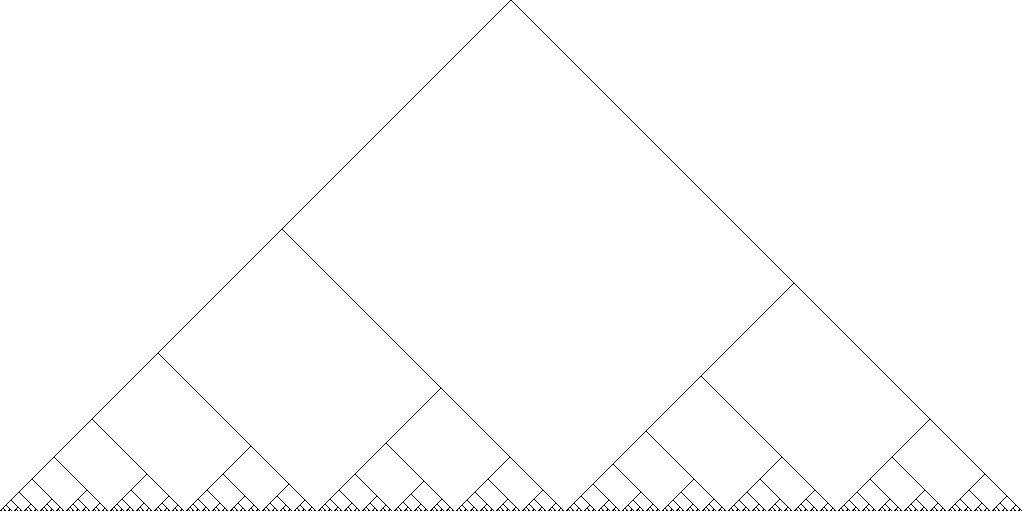
\includegraphics[width=\textwidth]{optimal.png}
    \caption{Optimal strategy for $e=512$, $\ell=2$.}
    \label{fig:optimal}
  \end{figure}
\end{frame}

%%

\begin{frame}{Implementation: constant time}
  \begin{itemize}
  \item Secret key sampling in constant time by \emph{restricting key
      space};
  \item $P + cQ$ in constant time via \emph{Montgomery ladder};
  \item Isogeny walk in constant time via \emph{any strategy}.
  \end{itemize}

  \begin{block}{Finite field operations in constant time}
    Only problem is to \emph{avoid inversions} as much as possible,
    but Vélu's formulas require one inversion per curve on the walk.

    \textbf{Solution\footcite{costello2016sidh}:} \emph{projectivize
      curve equations}
    \vspace{-4mm}
    \[E\;:\;\emph{CB}y^2 = \emph{C}x^3 + \emph{A}x^2 + \emph{C}x.\]
    \vspace{-0.9cm}
    \begin{itemize}
    \item Slightly increases operation counts of formulas;
    \item Delays all inversions to the very end;
    \item Only the value $(A:C)$ is needed in computations. Then:
      \[j(E) = \frac{256(A^2-3C^2)}{C^4(A^2-4C^2)}.\]
    \end{itemize}
  \end{block}
\end{frame}

%%

\begin{frame}{Summary}
  \emph{Public parameters:}
  \begin{itemize}
  \item $p = 2^a3^b - 1$,
  \item Staring curve $E\;:\; y^2 = x^3 + x$,
  \item Torsion generators
    \begin{gather*}
      P_A = (X_{a1}:Z_{a1}), \quad Q_A = (X_{a2}:Z_{a2}), \quad P_A-Q_A =  (X_{a3}:Z_{a3}),\\
      P_B = (X_{b1}:Z_{b1}), \quad Q_B = (X_{b2}:Z_{b2}), \quad P_B-Q_B =  (X_{b3}:Z_{b3}).
    \end{gather*}
  \end{itemize}

  \emph{Secret keys:}
  \begin{itemize}
  \item $R_A = P_A + cQ_A$ with $c\in[0,\dots,2^a-1]$,
  \item $R_B = P_A + cQ_A$ with $c\in[0,\dots,2^{b\lfloor\log_23\rfloor}-1]$.
  \end{itemize}

  \emph{Public keys (curve equation can be interpolated from three points):}
  \begin{itemize}
  \item $\phi(P_B), \phi(Q_B), \phi(P_B-Q_B)$,
  \item $\psi(P_A), \psi(Q_A), \psi(P_A-Q_A)$.
  \end{itemize}

  \emph{Shared secret:}
  \begin{itemize}
  \item $j = 256(A^2-3C^2)/C^4(A^2-4C^2)$.
  \end{itemize}
\end{frame}

%%

\begin{frame}
  \centering
  \begin{tikzpicture}
    \begin{scope}[xscale=1.2,black!60]
      \def\crater{7}
      \foreach \i in {1,...,\crater} {
        \draw[fill] (360/\crater*\i:3cm) circle (5pt);
        \draw (360/\crater*\i : 3cm) -- (360/\crater*\i+360/\crater : 3cm);
        \foreach \j in {-1,1} {
          \draw[fill] (360/\crater*\i : 3cm) -- (360/\crater*\i + \j*360/\crater/4 : 4cm) circle (3pt);
          \foreach \k in {-1,0,1} {
            \draw[fill] (360/\crater*\i + \j*360/\crater/4 : 4cm) --
            (360/\crater*\i + + \j*360/\crater/4 + \k*360/\crater/6 : 4.5cm) circle (1pt);
          }
        }
      }
    \end{scope}
    
    \draw (0,1) node{\Huge\bf Thank you};
    \draw (0,-0.6) node{\large\url{https://defeo.lu/}};
    \draw (0,-1.3) node{\large
\includegraphics[height=0.9em]{twitter.png}~\href{https://twitter.com/luca_defeo}{@luca\_defeo}};
  \end{tikzpicture}
\end{frame}

%% 

\begin{frame}[allowframebreaks]
  \frametitle{References}

  \defbibfilter{books}{\type{book} \or \type{booklet} \or \type{thesis}
    \or \type{report} \or \type{collection} \or \type{manual}
    \or \type{periodical} \or \type{proceedings}}
  \defbibfilter{articles}{\not \(\type{book} \or \type{booklet} \or \type{thesis}
    \or \type{report} \or \type{collection} \or \type{manual}
    \or \type{periodical} \or \type{proceedings}\)}

  \beamertemplatebookbibitems
  \printbibliography[filter=books]
  \beamertemplatearticlebibitems
  \printbibliography[filter=articles]
\end{frame}

\end{document}


% LocalWords:  Isogeny abelian isogenies hyperelliptic supersingular Frobenius
% LocalWords:  isogenous


